\documentclass[10pt,twocolumn]{article}

\usepackage[T1]{fontenc}
\usepackage{lmodern}
\usepackage[margin=0.62in,columnsep=0.24in]{geometry}
\usepackage{amsmath,amssymb,mathtools,bm}
\usepackage{booktabs,enumitem}
\usepackage{xcolor}
\usepackage{microtype}
\usepackage{tikz}
\usetikzlibrary{arrows.meta,positioning,calc,fit}
\usepackage[colorlinks=true,linkcolor=blue!45!black,
  citecolor=blue!45!black,urlcolor=blue!45!black]{hyperref}
\usepackage{fancyhdr}

\setlength{\parindent}{0.9em}
\setlength{\parskip}{0pt}
\setlength{\abovedisplayskip}{5pt}
\setlength{\belowdisplayskip}{5pt}
\setlength{\abovedisplayshortskip}{3pt}
\setlength{\belowdisplayshortskip}{3pt}
\setlength{\tabcolsep}{3.2pt}
\raggedbottom

\pagestyle{fancy}
\fancyhf{}
\fancyhead[L]{\footnotesize Fixed supported-FS Powell chart}
\fancyhead[R]{\footnotesize Canonical SR-SNAKE}
\fancyfoot[C]{\thepage}
\renewcommand{\headrulewidth}{0.25pt}

\newcommand{\ket}[1]{\lvert #1\rangle}
\newcommand{\bra}[1]{\langle #1\rvert}
\newcommand{\braket}[2]{\langle #1\mid #2\rangle}
\newcommand{\R}{\mathbb R}
\newcommand{\C}{\mathbb C}
\newcommand{\FS}{\mathrm{FS}}
\newcommand{\rank}{\operatorname{rank}}
\newcommand{\diag}{\operatorname{diag}}
\newcommand{\Span}{\operatorname{span}}
\newcommand{\conceptbreak}{%
  \par\medskip\noindent
  {\color{black!30}\rule{\columnwidth}{0.35pt}}%
  \par\medskip}
\newcommand{\micro}{\paragraph{Micro-intuition.}}
\newcommand{\mathderiv}{\paragraph{Mathematical derivation.}}
\newcommand{\commentaryblock}{\paragraph{Commentary.}}
\newcommand{\physical}{\paragraph{Physical interpretation.}}
\newcommand{\geometryblock}{\paragraph{Geometric visualization.}}
\newcommand{\impl}{\paragraph{Implementation translation.}}
\newcommand{\codeword}[1]{\texttt{\detokenize{#1}}}

\title{The Fixed Supported Fubini--Study Powell Chart\\
\large From a Binary-Padded Singleton to Canonical SR-SNAKE Optimization Coordinates}
\author{}
\date{16 July 2026}

\begin{document}
\maketitle
\vspace{-1.45em}

\begin{abstract}
This primer derives the canonical SR-SNAKE accepted-refit chart as one typed
composition whose governing question is concrete: after SR-SNAKE admits one
Pauli singleton, which numerical variables does Powell vary, and how does each
variation become a legal motion of the quantum state? A raw Pauli singleton
first becomes an exact legal-subspace generator under binary-padding
projection. This projection can enlarge the Pauli expansion: it adds companion
terms whose combined action preserves the encoded oscillator subspace. The
resulting Pauli components form one logical generator with one variational
angle and several expanded runtime entries. Block averaging maps those entries
to the shared logical angle, and block replication maps that angle back to the
executable array. Pulling the Fubini--Study metric through these maps reveals
which runtime mixtures generate distinct physical tangent motion. Spectral
support selects the resolved directions, and whitening rescales them into an
orthonormal physical tangent frame. Powell receives coordinates in that fixed
frame for one complete full-ansatz refit. The derivation follows this chain
through a three-level oscillator, the two-site Hubbard--Holstein register, a
complete numerical Gram example, the chart lifetime, implementation
certificates, a mastery quiz, and transfer problems.
\end{abstract}

\section*{The complete object-and-map architecture}

The construction begins with a truncated quantum model and ends with a scalar
energy supplied to Powell. Every arrow changes the representation of one
accepted variational displacement:
{\footnotesize
\begin{equation}
\begin{aligned}
 A
 &\xmapsto{\ \mathcal P A\mathcal P\ }
 \widetilde A
 \xmapsto{\ \text{one shared angle}\ }
 \bm\phi
 \xmapsto{\ R\ }
 \bm\vartheta,\\
 \bm\vartheta
 &\xmapsto{\ P\ }
 \bm\phi
 \xmapsto{\ T_\phi\ }
 T_{[\psi]}\mathcal M
 \xmapsto{\ \Re\langle\cdot,\cdot\rangle\ }
 G_\phi,\\
 G_\vartheta=P^{\mathsf T}G_\phi P
 &\xmapsto{\ \text{support}\ }
 (V_+,\Lambda_+)
 \xmapsto{\ O=V_+\Lambda_+^{-1/2}\ }
 z,\\
 z
 &\xmapsto{\ O\ }
 \delta\bm\vartheta
 \xmapsto{\ P\ }
 \delta\bm\phi
 \xmapsto{\ R\ }
 \widehat{\bm\vartheta}(z)
 \xmapsto{\ U\ }
 \ket{\psi(z)}
 \xmapsto{\ H}
 E(z).
\end{aligned}
\label{eq:architecture}
\end{equation}
}
Here \(\mathcal P\) is the projector onto the legal binary-boson subspace,
\(P\) averages expanded runtime blocks, \(R\) replicates logical angles,
\(T_\phi\) is the horizontal tangent map, \(G\) is its real Gram matrix,
\(O\) synthesizes supported orthonormal directions, and \(z\) is Powell's
coordinate vector. The same symbols retain these roles throughout the note.

Equation~\eqref{eq:architecture} should be read from left to right as one
accumulating construction. The first line changes an operator representation:
a raw qubit word becomes a legal grouped generator, and that generator acquires
one shared angle. The second line changes coordinate representations: expanded
runtime entries are gathered into logical angles, and logical angle
fluctuations are carried into the tangent space of the quantum state. The third
line equips those fluctuations with a physical length and chooses a resolved
orthonormal frame. The final line returns from that frame to an executable
circuit and then to a scalar energy. Thus every later object inherits the legal
action, shared-angle structure, and state-motion meaning established by the
earlier arrows.

\begin{center}
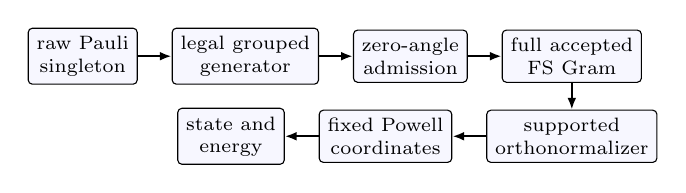
\begin{tikzpicture}[
  node distance=3.4mm and 4.3mm,
  every node/.style={font=\scriptsize,align=center},
  box/.style={draw,rounded corners=1.5pt,inner sep=3pt,fill=blue!3},
  arr/.style={-{Latex[length=1.5mm]},thick}
]
\node[box] (raw) {raw Pauli\\singleton};
\node[box,right=of raw] (legal) {legal grouped\\generator};
\node[box,right=of legal] (zero) {zero-angle\\admission};
\node[box,right=of zero] (gram) {full accepted\\FS Gram};
\node[box,below=of gram] (support) {supported\\orthonormalizer};
\node[box,left=of support] (powell) {fixed Powell\\coordinates};
\node[box,left=of powell] (energy) {state and\\energy};
\draw[arr] (raw)--(legal);
\draw[arr] (legal)--(zero);
\draw[arr] (zero)--(gram);
\draw[arr] (gram)--(support);
\draw[arr] (support)--(powell);
\draw[arr] (powell)--(energy);
\end{tikzpicture}
\end{center}

\physical The binary projector enforces the truncated oscillator model at the
operator level, so the first motion offered to the optimizer already belongs to
the intended finite bosonic Hilbert space. The logical/runtime maps then record
how one admitted physical generator is realized through several executable
Pauli factors under one shared variational amplitude.
Once every accepted generator has this shared-angle representation, the FS
Gram measures the state motion generated by their collective mixtures.
Whitening converts that measured geometry into Powell's numerical axes, making
each unit coordinate direction represent one unit of first-order motion of the
quantum ray at the accepted refit origin. The scalar energy sampled at the end
of the chain consequently belongs to the same ansatz family with which the
round began, expressed through a coordinate frame adapted to its local physical
geometry.

\conceptbreak

\section*{Part I. Binary padding defines the admissible singleton}

\subsection*{A truncated oscillator inside a binary register}

\micro A finite oscillator cutoff selects physical Fock levels inside a qubit
register whose dimension is a power of two.

\mathderiv Let \(n_{\max}\in\mathbb N\) be the maximum retained occupation.
The local physical dimension and qubit count are
\begin{equation}
d=n_{\max}+1,\qquad q=\left\lceil\log_2 d\right\rceil,\qquad
\mathcal H_q\simeq\C^{2^q}.
\label{eq:local-dimension}
\end{equation}
Binary encoding assigns the integer \(n\) to its \(q\)-bit codeword
\(b_q(n)\). The legal oscillator subspace and its orthogonal projector are
\begin{align}
\mathcal H_d
&=\Span\{\ket{b_q(n)}:0\leq n\leq n_{\max}\},\nonumber\\
\mathcal P_d
&=\sum_{n=0}^{n_{\max}}
\ket{b_q(n)}\bra{b_q(n)},\qquad
\mathcal P_d^2=\mathcal P_d=\mathcal P_d^\dagger.
\label{eq:legal-projector}
\end{align}
For \(L\) Hubbard--Holstein sites, the boson projector and complete-register
projector are
\begin{equation}
\mathcal P_B=\mathcal P_d^{\otimes L},\qquad
\mathcal P=\mathcal P_B\otimes I_F,
\label{eq:global-projector}
\end{equation}
where \(I_F\) acts on the \(2L\) fermionic qubits.

\commentaryblock A binary register supplies \(2^q\) basis codewords, because
each of its \(q\) qubits contributes two basis values. The truncated oscillator
supplies \(d=n_{\max}+1\) physical levels. Whenever \(d<2^q\), the encoding
places those \(d\) levels inside a larger computational space, leaving
\(2^q-d\) codewords as padding. The range of \(\mathcal P_d\) is precisely the
span of the encoded oscillator levels, and multiplication by \(\mathcal P_d\)
retains the component of a vector that lies in that span. An admissible state
therefore satisfies \(\mathcal P\ket\psi=\ket\psi\). Every Hamiltonian or
ansatz operation whose action closes on \(\operatorname{ran}\mathcal P\)
preserves this condition throughout the calculation.

\geometryblock The computational basis forms the vertices of a \(2^q\)-point
coordinate frame. The projector selects \(d\) vertices and the complex span
through them. A legal state is a vector inside that selected span. When the
projector acts on both sides of an operator, its right action selects the
operator's legal input columns and its left action selects the legal output
rows. This two-sided selection constructs an operator whose domain and image
both lie in the encoded oscillator space.

\conceptbreak

\subsection*{Exact projection of a raw Pauli singleton}

\micro A two-sided projector reconstructs the legal action of a raw Pauli word
and can express that reconstruction through a larger Pauli sum.

\mathderiv Let \(A=A^\dagger\) be one exposed Pauli direction. Define
\begin{equation}
\widetilde A=\mathcal P A\mathcal P.
\label{eq:projected-generator}
\end{equation}
The projected operator obeys
\begin{align}
\widetilde A^\dagger
&=(\mathcal P A\mathcal P)^\dagger
=\mathcal P A\mathcal P=\widetilde A,\nonumber\\
\mathcal P\widetilde A
&=\widetilde A=\widetilde A\mathcal P,\nonumber\\
(I-\mathcal P)\widetilde A\ket\psi
&=0\qquad(\mathcal P\ket\psi=\ket\psi).
\label{eq:projected-invariants}
\end{align}
Expand the legal operator in the Pauli basis on the complete register:
\begin{equation}
\widetilde A=\sum_{a=1}^{m}c_aP_a,\qquad
c_a=2^{-Q}\operatorname{Tr}(P_a\widetilde A)\in\R,
\label{eq:pauli-reexpansion}
\end{equation}
where \(Q\) is the total qubit count. The admitted finite-angle operation is
the grouped unitary
\begin{equation}
U_{\widetilde A}(\phi)=e^{-i\phi\widetilde A}.
\label{eq:grouped-unitary}
\end{equation}
Its legal-subspace invariance follows from the power series:
\begin{align}
\mathcal P e^{-i\phi\widetilde A}\mathcal P
&=\mathcal P\sum_{r=0}^{\infty}
\frac{(-i\phi)^r}{r!}\widetilde A^r\mathcal P\nonumber\\
&=\sum_{r=0}^{\infty}
\frac{(-i\phi)^r}{r!}\widetilde A^r\mathcal P
=e^{-i\phi\widetilde A}\mathcal P.
\label{eq:grouped-invariance}
\end{align}

\commentaryblock The matrix \(\mathcal P A\mathcal P\) can contain fewer
transitions and more Pauli terms than the original word \(A\). These statements
describe two different representations of the same construction. In the
computational-basis matrix, the projectors select legal input and output
transitions. In the Pauli basis, reproducing that selected matrix can require
adding companion words to the original Pauli proposal. Their coefficients are
fixed by Eq.~\eqref{eq:pauli-reexpansion}; they are components of one operator,
so they acquire one shared variational angle.

\physical The raw word proposes transitions throughout the qubit embedding
space. The two-sided projector reconstructs the part of that action connecting
physical Fock levels, and Pauli re-expansion turns the reconstructed matrix
into executable qubit operators. A newly added companion term can agree with
the raw word on legal transitions and oppose it on a padding transition. Their
sum thereby preserves the desired physical motion and cancels the illegal
motion. This constructive enlargement of the Pauli representation is the
mechanism by which one exposed singleton becomes a padding-safe grouped
generator.

\impl Canonical child preparation performs Eq.~\eqref{eq:projected-generator}
before Phase-I child scoring and before projected-identity deduplication. A
zero projected polynomial closes the candidate path. A surviving polynomial
receives grouped-exact execution metadata and enters selection as one logical
singleton.

\conceptbreak

\subsection*{Toy example: \(n_{\max}=2\) on two qubits}

\micro Binary encoding writes each oscillator occupation as a fixed-width
string of qubit values. The unused string becomes the padding state.

\commentaryblock A \emph{codeword} is the fixed-width bit string assigned to
one basis state by an encoder. For two qubits, the computational-basis
codewords are \(00\), \(01\), \(10\), and \(11\). The right bit \(q_0\)
is the ones place, the left bit \(q_1\) is the twos place, and
\[
n=2q_1+q_0,\qquad q_1,q_0\in\{0,1\}.
\]
The leading zero in \(00\) records the state of the second qubit. Thus the
integer zero has the two-qubit representation \(00\), just as the decimal
integer two has the binary representation \(10\).

This notation carries two descriptions at once. The integer \(n\) names an
oscillator occupation in the three-dimensional Fock basis. The codeword
\(q_1q_0\) names the qubit state used to store that occupation inside a
four-dimensional register. The encoder \(B\) below is the typed map connecting
these descriptions; it changes the representation of a basis state and
preserves which physical oscillator level the state denotes.

\mathderiv Let \(B\) be the encoding map from the three retained oscillator
basis states into the two-qubit register:
\begin{equation*}
B\ket{n}=\ket{b_2(n)}.
\end{equation*}
Here \(b_2(n)\) is the two-bit binary codeword for the integer \(n\). Since
\(d=3\) and \(q=2\), the encoded basis map is
\begin{equation}
B\ket{0}=\ket{00},\qquad
B\ket{1}=\ket{01},\qquad
B\ket{2}=\ket{10}.
\label{eq:qutrit-codes}
\end{equation}
The ket on the left names an abstract oscillator occupation. The ket on the
right names the corresponding state of two physical qubits. The complete
assignment is
\begin{center}
\renewcommand{\arraystretch}{1.08}
\begin{tabular}{@{}ccc@{}}
\toprule
Integer & Two-qubit word & Role at \(n_{\max}=2\) \\
\midrule
\(0\) & \(00\) & encoded \(\ket0\) \\
\(1\) & \(01\) & encoded \(\ket1\) \\
\(2\) & \(10\) & encoded \(\ket2\) \\
\(3\) & \(11\) & padding word \\
\bottomrule
\end{tabular}
\end{center}

\micro The legal-subspace projector is constructed first; the raw Pauli
singleton is then passed through that projector to produce the grouped
generator.

\mathderiv With Pauli labels ordered as \(q_1q_0\), the rank-three
legal-subspace projector is
\begin{align}
\mathcal P_3
&=I-\ket{11}\bra{11}\nonumber\\
&=I-\frac14(I-Z_1)(I-Z_0)\nonumber\\
&=\frac14(3I+Z_1+Z_0-Z_1Z_0).
\label{eq:qutrit-projector-pauli}
\end{align}
Equation~\eqref{eq:qutrit-projector-pauli} defines a projector: it preserves
\(\ket{00}\), \(\ket{01}\), and \(\ket{10}\), and it sends the padding word
\(\ket{11}\) to the zero vector. The subscript \(3\) records the dimension of
its image.

Now choose the raw Pauli singleton
\begin{equation*}
A=I_1X_0.
\end{equation*}
The symbol \(I_1\) leaves qubit \(q_1\) unchanged, and \(X_0\) flips qubit
\(q_0\). Therefore
\begin{align*}
A\ket{00}&=\ket{01},& A\ket{01}&=\ket{00},\\
A\ket{10}&=\ket{11},& A\ket{11}&=\ket{10}.
\end{align*}
The projector \(\mathcal P_3\) and raw singleton \(A\) are separate operators
with separate roles. The projector selects the encoded oscillator subspace.
The singleton proposes a variational transition. Their composition produces
the padding-respecting generator:
\begin{align}
\widetilde A
&=\mathcal P_3(I_1X_0)\mathcal P_3\nonumber\\
&=\ket{00}\bra{01}+\ket{01}\bra{00}\nonumber\\
&=\left(\frac{I_1+Z_1}{2}\right)X_0
=\frac12(I_1X_0+Z_1X_0).
\label{eq:qutrit-projected-x}
\end{align}
Thus Eq.~\eqref{eq:qutrit-projector-pauli} constructs the projector.
Equation~\eqref{eq:qutrit-projected-x} constructs the generator. The two Pauli
terms in \(\widetilde A\) form one grouped generator and share one logical
variational angle.
The added companion term can be followed directly on the most-significant
qubit:
\begin{align}
\frac12(I_1+Z_1)\ket{0}_{q_1}
&=\ket{0}_{q_1},\nonumber\\
\frac12(I_1+Z_1)\ket{1}_{q_1}
&=0.
\label{eq:qutrit-companion-action}
\end{align}
On codewords with \(q_1=0\), the two Pauli terms agree and their
one-half coefficients sum to the original \(X_0\) flip. On codewords with
\(q_1=1\), \(Z_1X_0\) has the opposite sign from \(I_1X_0\), so the two
one-half contributions sum to zero. Projection has therefore \emph{added}
\(Z_1X_0\) to the Pauli representation; the action of the enlarged sum
preserves \(00\leftrightarrow01\) and cancels
\(10\leftrightarrow11\).
On a general legal state
\(\ket\psi=a\ket{00}+b\ket{01}+c\ket{10}\),
\begin{equation}
\widetilde A\ket\psi=b\ket{00}+a\ket{01},
\label{eq:qutrit-action}
\end{equation}
which lies in \(\mathcal H_3\).

\begin{center}
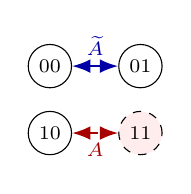
\begin{tikzpicture}[
  every node/.style={font=\scriptsize},
  state/.style={circle,draw,minimum size=5.5mm,inner sep=0pt},
  arr/.style={<->,>=Latex,thick}
]
\node[state] (s0) at (0,0) {$00$};
\node[state] (s1) at (1.15,0) {$01$};
\node[state] (s2) at (0,-0.85) {$10$};
\node[state,fill=red!7,dashed] (s3) at (1.15,-0.85) {$11$};
\draw[arr,blue!65!black] (s0)--node[above]{$\widetilde A$}(s1);
\draw[arr,dashed,red!65!black] (s2)--node[below]{$A$}(s3);
\end{tikzpicture}
\end{center}

\commentaryblock The projection has changed one raw Pauli word into the
two-term polynomial
\(\tfrac12I_1X_0+\tfrac12Z_1X_0\). This is constructive addition at the level
of the Pauli expansion. The resulting matrix action contains the desired
\(00\leftrightarrow01\) transition because the two terms reinforce one
another there, and it contains zero amplitude for the
\(10\leftrightarrow11\) transition because the two terms oppose one another
there. Grouped execution preserves their fixed relative coefficients at finite
angle. The complete sum is one generator, its exponential is one logical
unitary family, and its executable representation supplies a two-entry runtime
block controlled by one shared logical coordinate.

\conceptbreak

\subsection*{Paper-I Hubbard--Holstein register examples}

\micro Local projection embeds directly into the complete fermion-boson Pauli
word.

\mathderiv For \(L=2\), the fermion register has four qubits. At
\(n_{\max}=2\), each boson site has two qubits, so
\begin{equation}
Q=2L+L\left\lceil\log_2(n_{\max}+1)\right\rceil
=4+2(2)=8.
\label{eq:hh-eight-qubits}
\end{equation}
The repository word order is \(q_{Q-1}\cdots q_0\), with the boson blocks on
the left and the fermion block on the right. The tested raw child and its exact
projection are
\begin{align}
 A&=\codeword{eeexeeee},\nonumber\\
\widetilde A
&=\frac12\codeword{eeexeeee}
+\frac12\codeword{eezxeeee}.
\label{eq:hh-nph2-projection}
\end{align}
In these strings, \codeword{e} denotes the identity operator, and the letters
are written left to right from the largest qubit index to qubit \(0\). The four
rightmost identities act on the fermion register. The boson substring
\codeword{eeex} contains one local \codeword{ex} flip. Projection adds the
companion string \codeword{eezx}; the two strings reinforce the legal
least-significant-bit transition and oppose the transition entering the local
padding word.

For \(n_{\max}=4\), each site contains \(d=5\) levels in three qubits, giving
\begin{equation}
Q=4+2(3)=10.
\label{eq:hh-ten-qubits}
\end{equation}
One tested local least-significant-bit flip obeys
\begin{align}
A&=\codeword{eexeeeeeee},\nonumber\\
\widetilde A
&=\frac12\codeword{eexeeeeeee}
+\frac12\codeword{zexeeeeeee}.
\label{eq:hh-nph4-projection}
\end{align}
The local three-qubit identity
\begin{equation}
\mathcal P_5(I_2I_1X_0)\mathcal P_5
=\frac12(I_2+Z_2)I_1X_0
\label{eq:five-level-projected-x}
\end{equation}
retains the \(0\leftrightarrow1\) and \(2\leftrightarrow3\) transitions. The
level \(4\) amplitude remains stationary under this projected direction.

\physical The full-register strings show that padding is a local boson
constraint embedded inside a fermion-boson ansatz. Identities on the remaining
sites and fermionic qubits carry those subsystems unchanged through this local
generator. Projection can increase the Pauli-term count of one candidate,
because the Pauli basis needs several words to reproduce the selected
legal-subspace matrix. That increased count becomes the runtime multiplicity of
one logical coordinate: the circuit layer contains several executable factors,
and their variational meaning remains tied to the single projected bosonic
motion from which they arose. The local toy construction therefore scales
directly into the complete Hubbard--Holstein register.

\conceptbreak

\section*{Part II. One projected generator creates one logical coordinate}

\subsection*{Logical blocks and expanded runtime arrays}

\micro A grouped generator carries one variational angle across every Pauli
factor in its executable representation.

The projected generator \(\widetilde A=\sum_a c_aP_a\) is a single
mathematical direction, yet its circuit realization presents a list of Pauli
factors to the runtime. We shall call each position in that executable list a
\emph{runtime entry}. The logical coordinate records the amplitude of the
projected generator as a whole; the runtime entries record where that shared
amplitude is written for circuit construction and optimization plumbing.

\mathderiv Let the accepted ansatz contain \(d\) logical generators. Generator
\(\ell\) expands into \(m_\ell\) runtime factors with index block
\(I_\ell\), and \(m=\sum_{\ell=1}^d m_\ell\). Define
\begin{equation}
\bm\phi=(\phi_1,\ldots,\phi_d)^{\mathsf T}\in\R^d,\qquad
\bm\vartheta\in\R^m.
\label{eq:logical-runtime-types}
\end{equation}
The block-average map \(P:\R^m\to\R^d\) and uniform lift
\(R:\R^d\to\R^m\) have entries
\begin{equation}
P_{\ell j}=
\begin{cases}
m_\ell^{-1},&j\in I_\ell,\\
0,&j\notin I_\ell,
\end{cases}
\quad
R_{j\ell}=
\begin{cases}
1,&j\in I_\ell,\\
0,&j\notin I_\ell.
\end{cases}
\label{eq:block-maps}
\end{equation}
Their compositions satisfy
\begin{align}
PR&=I_d,\nonumber\\
Q&=RP,\qquad Q^2=Q,\qquad \operatorname{im}Q=\operatorname{im}R,\nonumber\\
\ker Q&=\ker P.
\label{eq:block-map-identities}
\end{align}
State preparation uses the projected runtime array
\begin{equation}
\widehat{\bm\vartheta}=RP\bm\vartheta=R\bm\phi,\qquad
\bm\phi=P\bm\vartheta.
\label{eq:runtime-state-map}
\end{equation}

\commentaryblock The entries inside one runtime block may begin as distinct
numbers. The map \(P\) extracts their mean, and \(R\) writes that mean into
every position of the block. The projector \(Q=RP\) selects the uniform block
subspace. A vector in \(\ker P\) redistributes values inside blocks with zero
change in every block mean.

For example, suppose the second logical generator occupies runtime entries
\(2\) and \(3\). Then
\begin{equation}
\begin{bmatrix}\vartheta_2\\\vartheta_3\end{bmatrix}
\xmapsto{\ P\ }
\phi_2=\frac{\vartheta_2+\vartheta_3}{2}
\xmapsto{\ R\ }
\begin{bmatrix}\phi_2\\\phi_2\end{bmatrix}.
\label{eq:one-block-example}
\end{equation}
The first arrow gathers an expanded representation into its shared logical
amplitude. The second arrow produces the executable representative in which
both entries carry that amplitude. Consequently, the pair
\((\vartheta_2,\vartheta_3)\) describes one circuit state through its mean, and
the difference \((1,-1)\) is an internal redistribution of the expanded array.

\geometryblock The expanded runtime space \(\R^m\) contains a \(d\)-dimensional
uniform-block plane \(\operatorname{im}R\). Each fiber
\(P^{-1}(\bm\phi)=R\bm\phi+\ker P\) contains all expanded arrays representing
the same logical angles. Circuit evaluation collapses each fiber to its uniform
representative \(R\bm\phi\).

\conceptbreak

\subsection*{Zero-growth admission}

\micro Singleton admission enlarges the coordinate registry and preserves the
accepted state through a zero new angle.

\mathderiv Suppose the current registry has logical angles
\(\bm\phi_k\in\R^{d_k}\). The projected candidate
\(\widetilde A_r=\sum_{a=1}^{m_r}c_aP_a\) becomes logical block \(d_k+1\).
The enlarged origin is
\begin{align}
\bm\phi_{k,+}^{(0)}
&=\begin{bmatrix}\bm\phi_k\\0\end{bmatrix}
\in\R^{d_k+1},\nonumber\\
\bm\vartheta_{k,+}^{(0)}
&=R_{k,+}\bm\phi_{k,+}^{(0)}
\in\R^{m_k+m_r}.
\label{eq:zero-growth-origin}
\end{align}
If the admitted unitary is inserted at its selected position, then
\begin{align}
U_{k,+}(\bm\phi_{k,+}^{(0)})
&=U_{>r}e^{-i0\widetilde A_r}U_{<r}
=U_{>r}U_{<r},\nonumber\\
\ket{\psi_{k,+}^{(0)}}&=\ket{\psi_k},\qquad
E_{k,+}^{(0)}=E_k.
\label{eq:zero-growth-state}
\end{align}
The derivative in the new coordinate is
\begin{equation}
\left.\partial_{\phi_r}\ket{\psi_{k,+}}\right|_{\bm\phi_{k,+}^{(0)}}
=-iU_{>r}\widetilde A_rU_{<r}\ket{\psi_{\rm ref}}.
\label{eq:new-candidate-tangent}
\end{equation}

\physical Admission adds a new direction to the variational manifold at the
current quantum ray. Zero initialization anchors the enlarged ansatz at the
state already accepted by the preceding round, preserving its state and energy
exactly. This common anchor makes the comparison meaningful: the newly
available coordinate begins with zero displacement, and every subsequent
energy change comes from refitting the enlarged manifold. The new derivative
records the infinitesimal state motion available from the projected singleton.
A full accepted-ansatz refit then lets every old logical angle and the new
angle move together, so the admitted direction can cooperate with the entire
accepted coordinate set.

\impl Binary projection precedes Eq.~\eqref{eq:zero-growth-origin}. Therefore,
the projected polynomial determines \(m_r\), the new runtime slice, the
logical-to-runtime registry, and the columns used to form the accepted-refit
Gram matrix. The registry is consequently part of the mathematical chart: it
specifies which runtime entries belong to each logical generator and thereby
fixes the matrices \(P\) and \(R\).

\conceptbreak

\section*{Part III. Fubini--Study geometry measures physical state motion}

\subsection*{Horizontal tangent vectors}

\micro Projective geometry selects the infinitesimal component orthogonal to
the state and measures the motion of the quantum ray.

A normalized vector \(\ket\psi\) contains one representational freedom:
\(e^{i\alpha}\ket\psi\) denotes the same physical pure state for every real
phase \(\alpha\). The physical state is therefore the ray
\([\psi]=\{e^{i\alpha}\ket\psi:\alpha\in\R\}\). A parameter derivative can
contain a component that changes this phase representative and a component that
moves the ray itself. The horizontal projector below extracts the second
component, so the ensuing Gram matrix measures physically distinguishable
first-order motion.

\mathderiv Let
\begin{equation}
\ket{\psi(\bm\phi)}=U(\bm\phi)\ket{\psi_{\rm ref}},\qquad
\braket{\psi}{\psi}=1.
\label{eq:normalized-state}
\end{equation}
At the zero-growth origin \(\bm\phi^{(0)}\), define
\begin{align}
\Pi&=I-\ket\psi\bra\psi,\nonumber\\
\ket{t_\ell}&=\Pi\ket{\partial_\ell\psi}
=\ket{\partial_\ell\psi}
-\ket\psi\braket{\psi}{\partial_\ell\psi},\nonumber\\
T_\phi&=[\ket{t_1},\ldots,\ket{t_d}]
:\R^d\longrightarrow T_{[\psi]}\mathcal M.
\label{eq:horizontal-tangents}
\end{align}
For \(\delta\bm\phi\in\R^d\), the represented horizontal tangent is
\begin{equation}
\ket{\delta\psi_\perp}=T_\phi\delta\bm\phi
=\sum_{\ell=1}^{d}\delta\phi_\ell\ket{t_\ell}.
\label{eq:tangent-combination}
\end{equation}
Its squared real norm is
\begin{align}
\|\delta\psi_\perp\|_{\R}^2
&=\Re\braket{\delta\psi_\perp}{\delta\psi_\perp}\nonumber\\
&=\sum_{\ell,s}\delta\phi_\ell
\Re\braket{t_\ell}{t_s}\delta\phi_s\nonumber\\
&=\delta\bm\phi^{\mathsf T}G_\phi\delta\bm\phi,
\qquad
G_\phi=\Re(T_\phi^\dagger T_\phi).
\label{eq:logical-fs-gram}
\end{align}
Equivalently,
\begin{equation}
(G_\phi)_{\ell s}
=\Re\!\left[
\braket{\partial_\ell\psi}{\partial_s\psi}
-\braket{\partial_\ell\psi}{\psi}
 \braket{\psi}{\partial_s\psi}
\right].
\label{eq:fs-components}
\end{equation}

\commentaryblock The rank-one operator \(\ket\psi\bra\psi\) selects the
component parallel to the current state. Subtracting it from the identity gives
\(\Pi\), which retains the orthogonal component of each parameter derivative.
The vectors \(\ket{t_\ell}\) are therefore concrete horizontal
representatives of projective tangent directions. Their complex Hilbert-space
inner products contain real symmetric length information and imaginary
antisymmetric phase information. Taking the real part builds the Riemannian
metric used here. The resulting Gram matrix is positive semidefinite because
every quadratic form
\(\delta\bm\phi^{\mathsf T}G_\phi\delta\bm\phi\) is the squared norm of the
horizontal tangent \(T_\phi\delta\bm\phi\).

\physical A parameter displacement is a list of angle changes. Multiplication
by \(T_\phi\) turns that list into an infinitesimal many-body state change.
Multiplication by \(G_\phi\) evaluates lengths and angles between such changes.
The diagonal of \(G_\phi\) records how strongly each isolated angle moves the
state, and the off-diagonal entries record constructive or opposing overlap
between pairs of angle-induced motions. Thus two large parameter changes can
produce a small physical displacement when their tangent vectors nearly
cancel, and two numerically different coordinates can represent comparable
state motion after metric rescaling. This local physical scale supplies the
geometry used to condition the Powell search.

\geometryblock Picture the normalized state vectors as points on a sphere.
Multiplication by a global phase moves along a circle of equivalent
representatives above one physical ray. The projector \(\Pi\) selects the
tangent plane orthogonal to that phase circle. The resulting tangent vectors lie in a
horizontal plane, and \(G_\phi\) records their lengths and mutual angles in the
parameter-coordinate basis.

\conceptbreak

\subsection*{Pulling the metric into expanded runtime coordinates}

\micro The block-average map transfers logical FS geometry into the expanded
runtime representation.

\mathderiv A runtime displacement obeys
\begin{equation}
\delta\bm\phi=P\delta\bm\vartheta.
\label{eq:runtime-to-logical-displacement}
\end{equation}
The chain rule yields
\begin{align}
T_\vartheta
&=T_\phi P,\nonumber\\
G_\vartheta
&=\Re(T_\vartheta^\dagger T_\vartheta)
=P^{\mathsf T}G_\phi P.
\label{eq:runtime-pullback}
\end{align}
The physical length is representation-consistent:
\begin{align}
\delta\bm\vartheta^{\mathsf T}G_\vartheta
\delta\bm\vartheta
&=\delta\bm\vartheta^{\mathsf T}P^{\mathsf T}G_\phi
P\delta\bm\vartheta\nonumber\\
&=\delta\bm\phi^{\mathsf T}G_\phi\delta\bm\phi
=\|T_\phi\delta\bm\phi\|_{\R}^2.
\label{eq:pullback-length}
\end{align}
Every alias \(a\in\ker P\) satisfies
\begin{equation}
Pa=0,\qquad T_\vartheta a=0,\qquad G_\vartheta a=0.
\label{eq:alias-nullity}
\end{equation}

\commentaryblock Equation~\eqref{eq:runtime-pullback} is the chain rule for a
metric. The map \(P\) first converts a runtime fluctuation into the logical
angle fluctuation seen by the state, and \(T_\phi\) then converts that logical
fluctuation into a horizontal state tangent. Their composition is
\(T_\vartheta=T_\phi P\). Taking its Gram matrix places one copy of \(P\) on
each side of \(G_\phi\), yielding \(P^{\mathsf T}G_\phi P\). An alias vector
belongs to \(\ker P\), so it describes a redistribution among runtime entries
whose shared logical angles remain fixed. Its zero FS length expresses
representational redundancy inside the expanded array.

\geometryblock The logical FS unit sphere pulls back to a cylinder-like
quadratic surface in expanded runtime space. The surface has zero curvature
along each alias fiber \(\ker P\), because movement along a fiber preserves
the logical angle and quantum state. The positive directions describe genuine
state motion; support factorization identifies their span.

\begin{center}
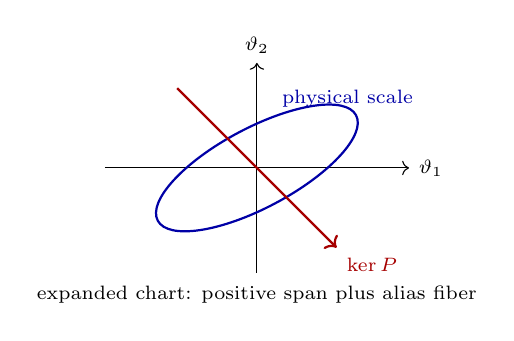
\begin{tikzpicture}[scale=0.92,
  every node/.style={font=\scriptsize},
  arr/.style={-{Latex[length=1.5mm]},thick}]
\draw[->] (-2.1,0)--(2.1,0) node[right]{$\vartheta_1$};
\draw[->] (0,-1.45)--(0,1.45) node[above]{$\vartheta_2$};
\draw[blue!65!black,thick,rotate=28] (0,0) ellipse (1.55 and 0.55);
\draw[red!65!black,thick,->] (-1.1,1.1)--(1.1,-1.1)
 node[below right]{$\ker P$};
\node[blue!65!black] at (1.25,0.95) {physical scale};
\node at (0,-1.75) {expanded chart: positive span plus alias fiber};
\end{tikzpicture}
\end{center}

\conceptbreak

\section*{Part IV. Spectral support and whitening}

\subsection*{Support is the physically resolved tangent quotient}

\micro Spectral support retains metric modes with certified positive physical
length.

An eigenmode of \(G_\vartheta\) is a particular mixture of runtime-coordinate
directions whose FS length scale is reproduced by a single number. If
\(G_\vartheta v_a=\lambda_av_a\) and \(\|v_a\|_2=1\), then a displacement
\(\eta v_a\) has squared first-order FS length
\(\eta^2\lambda_a\). The eigenvector \(v_a\) therefore identifies the mixture,
and the eigenvalue \(\lambda_a\) quantifies how strongly that mixture moves the
quantum ray.

\mathderiv Symmetrize and diagonalize the expanded Gram matrix:
\begin{equation}
G_\vartheta=V\Lambda V^{\mathsf T},\qquad
\Lambda=\diag(\lambda_1,\ldots,\lambda_m),\qquad
V^{\mathsf T}V=I_m.
\label{eq:gram-spectrum}
\end{equation}
Let \(\lambda_{\max}^+\) be its largest positive eigenvalue and define
\begin{equation}
\mathcal I_+=\{a:\lambda_a>\tau_G\lambda_{\max}^+\}.
\label{eq:support-index}
\end{equation}
Collect the retained eigenvectors and eigenvalues as
\begin{equation}
V_+\in\R^{m\times r},\qquad
\Lambda_+\in\R^{r\times r},\qquad
r=|\mathcal I_+|.
\label{eq:supported-factors}
\end{equation}
They satisfy
\begin{equation}
G_\vartheta V_+=V_+\Lambda_+,\qquad
V_+^{\mathsf T}V_+=I_r,\qquad
\Lambda_+\succ0.
\label{eq:supported-eigenproblem}
\end{equation}
The supported runtime displacement space is
\begin{equation}
\mathcal S=\operatorname{im}V_+\simeq
\R^m/\ker G_\vartheta.
\label{eq:supported-quotient}
\end{equation}

\commentaryblock The threshold \(\tau_G\) is a numerical support certificate.
It compares each eigenvalue with the largest positive scale and retains modes
whose physical length is resolved at the declared relative precision. The
retained columns of \(V_+\) span the supported tangent-coordinate plane.
Directions in the metric kernel produce zero horizontal motion, so the quotient
\(\R^m/\ker G_\vartheta\) groups runtime arrays that represent the same
physical tangent. The subspace \(\operatorname{im}V_+\) supplies one
minimum-Euclidean-norm representative for each resolved quotient class.
Consequently, support performs two related operations: it acknowledges the
equivalence created by runtime aliases and it protects the numerical
construction from treating unresolved metric scales as trustworthy axes.

\geometryblock Imagine compressing every affine alias fiber to one point. The
expanded runtime space then becomes a lower-dimensional physical tangent
coordinate space. The columns of \(V_+\) choose orthonormal Euclidean axes in
that supported representative plane, and \(\Lambda_+\) records their physical
FS scales.

\conceptbreak

\subsection*{The exact supported-FS orthonormalizer}

\micro Whitening rescales supported eigenmodes so Euclidean length in Powell
coordinates equals FS tangent length at the origin.

\mathderiv Define the synthesis and analysis maps
\begin{align}
O&=V_+\Lambda_+^{-1/2}:\R^r\longrightarrow\R^m,\nonumber\\
L&=\Lambda_+^{1/2}V_+^{\mathsf T}:\R^m\longrightarrow\R^r.
\label{eq:analysis-synthesis-maps}
\end{align}
Their supported identities are
\begin{align}
O^{\mathsf T}G_\vartheta O
&=\Lambda_+^{-1/2}V_+^{\mathsf T}
G_\vartheta V_+\Lambda_+^{-1/2}=I_r,\nonumber\\
LO&=I_r,\nonumber\\
OL&=V_+V_+^{\mathsf T}.
\label{eq:whitening-identities}
\end{align}
For \(z\in\R^r\), set
\begin{equation}
\delta\bm\vartheta_+=Oz,\qquad
\delta\bm\phi=POz.
\label{eq:whitened-lifts}
\end{equation}
Then
\begin{align}
\delta\bm\vartheta_+^{\mathsf T}G_\vartheta
\delta\bm\vartheta_+
&=z^{\mathsf T}O^{\mathsf T}G_\vartheta Oz
=z^{\mathsf T}z,\nonumber\\
T_\vartheta\delta\bm\vartheta_+
&=T_\vartheta Oz.
\label{eq:whitened-length}
\end{align}
The physical frame
\begin{equation}
\mathcal E=T_\vartheta O
\label{eq:physical-frame}
\end{equation}
obeys
\begin{equation}
\Re(\mathcal E^\dagger\mathcal E)=I_r.
\label{eq:physical-frame-orthonormal}
\end{equation}

\commentaryblock The factor \(\Lambda_+^{-1/2}\) divides eigenmode \(v_a\) by
\(\sqrt{\lambda_a}\). Since \(v_a\) originally has squared FS length
\(\lambda_a\), the rescaled direction
\(v_a/\sqrt{\lambda_a}\) has squared FS length one. The matrix \(O\) performs
this operation for every supported eigenmode at once. Its columns live in the
expanded runtime space, and the product \(PO\) gathers those columns into
logical-angle displacements. Equation~\eqref{eq:whitening-identities} then
certifies that ordinary Euclidean dot products in \(z\)-space reproduce the
FS inner product at the chart origin.

\physical Each component \(z_a\) is the amplitude of one orthonormal
horizontal state-motion mode. A unit step along any coordinate axis has unit
first-order FS length at the origin, so Powell begins with axes calibrated by
how far they move the quantum ray. A raw parameter direction that moves the
state strongly receives a smaller numerical coefficient through
\(\lambda_a^{-1/2}\); a resolved direction that moves the state gently receives
a larger coefficient. The nonlinear circuit and Hamiltonian still determine
the energy along each displacement. Thus whitening equalizes the local
kinematic scale of state motion and lets the objective reveal the remaining
energetic stiffness, coupling, and higher-order response.

\geometryblock The supported metric defines an ellipsoid in runtime
coordinates: equal-FS-length displacements lie on its surface. The eigenvectors
give the principal axes of this ellipsoid, and the square roots of the
eigenvalues give their inverse coordinate radii. The map \(O\) sends the
Euclidean unit sphere in \(z\)-space onto that ellipsoid. Powell therefore sees
a sphere at the origin. The same physical neighborhood appears anisotropic in
raw runtime coordinates.

\conceptbreak

\section*{Part V. Complete numerical toy chart}

\subsection*{One old generator and one projected two-term singleton}

\micro A \(3\)-entry runtime array with two logical angles contains one exact
alias and two physical tangent directions.

\mathderiv Let logical block \(1\) have one runtime factor and let the projected
singleton from Eq.~\eqref{eq:qutrit-projected-x} have two runtime factors.
Then
\begin{equation}
I_1=\{1\},\qquad I_2=\{2,3\},\qquad
\bm\phi=\begin{bmatrix}\phi_1\\\phi_2\end{bmatrix},\qquad
\bm\vartheta=\begin{bmatrix}\vartheta_1\\\vartheta_2\\\vartheta_3\end{bmatrix}.
\label{eq:toy-blocks}
\end{equation}
The block maps are
\begin{equation}
P=
\begin{bmatrix}
1&0&0\\
0&\tfrac12&\tfrac12
\end{bmatrix},\qquad
R=
\begin{bmatrix}
1&0\\
0&1\\
0&1
\end{bmatrix}.
\label{eq:toy-pr}
\end{equation}
Direct multiplication gives
\begin{align}
PR&=
\begin{bmatrix}1&0\\0&1\end{bmatrix},\nonumber\\
RP&=
\begin{bmatrix}
1&0&0\\
0&\tfrac12&\tfrac12\\
0&\tfrac12&\tfrac12
\end{bmatrix}.
\label{eq:toy-projector}
\end{align}
The uniform candidate direction and its alias are
\begin{equation}
s=\frac1{\sqrt2}\begin{bmatrix}0\\1\\1\end{bmatrix},\qquad
a=\frac1{\sqrt2}\begin{bmatrix}0\\1\\-1\end{bmatrix},\qquad
Pa=0.
\label{eq:toy-uniform-alias}
\end{equation}

Assume the two logical tangents are orthogonal at the accepted origin with
lengths \(2\) and \(3\):
\begin{equation}
G_\phi=
\begin{bmatrix}4&0\\0&9\end{bmatrix}.
\label{eq:toy-logical-gram}
\end{equation}
The expanded pullback is
\begin{align}
G_\vartheta
&=P^{\mathsf T}G_\phi P\nonumber\\
&=\begin{bmatrix}
4&0&0\\
0&\tfrac94&\tfrac94\\
0&\tfrac94&\tfrac94
\end{bmatrix}.
\label{eq:toy-runtime-gram}
\end{align}
Its eigensystem can be read directly:
\begin{equation}
\begin{array}{c|c}
\lambda&v\\ \hline
4&(1,0,0)^{\mathsf T}\\
\tfrac92&(0,1,1)^{\mathsf T}/\sqrt2\\
0&(0,1,-1)^{\mathsf T}/\sqrt2
\end{array}
\label{eq:toy-eigensystem}
\end{equation}
Therefore
\begin{equation}
V_+=
\begin{bmatrix}
1&0\\
0&1/\sqrt2\\
0&1/\sqrt2
\end{bmatrix},\qquad
\Lambda_+=
\begin{bmatrix}
4&0\\0&9/2
\end{bmatrix},
\label{eq:toy-supported-factors}
\end{equation}
and
\begin{align}
O=V_+\Lambda_+^{-1/2}
&=\begin{bmatrix}
\tfrac12&0\\
0&\tfrac13\\
0&\tfrac13
\end{bmatrix},\nonumber\\
PO&=\begin{bmatrix}
\tfrac12&0\\
0&\tfrac13
\end{bmatrix}.
\label{eq:toy-orthonormalizer}
\end{align}
For \(z=(z_1,z_2)^{\mathsf T}\),
\begin{align}
\delta\bm\vartheta_+
&=Oz
=\begin{bmatrix}z_1/2\\z_2/3\\z_2/3\end{bmatrix},\nonumber\\
\delta\bm\phi
&=POz
=\begin{bmatrix}z_1/2\\z_2/3\end{bmatrix},\nonumber\\
\delta\bm\vartheta_+^{\mathsf T}G_\vartheta
\delta\bm\vartheta_+
&=z_1^2+z_2^2.
\label{eq:toy-final-map}
\end{align}

\commentaryblock The matrices can now be read as a record of the entire
construction. Columns \(2\) and \(3\) of \(G_\vartheta\) are equal because
runtime entries \(2\) and \(3\) carry one shared logical angle. Their
difference vector \(a=(0,1,-1)^{\mathsf T}/\sqrt2\) is consequently an exact
zero-eigenvalue mode. Their sum vector
\(s=(0,1,1)^{\mathsf T}/\sqrt2\) is the physical candidate direction; its
expanded-coordinate eigenvalue is \(9/2\), reflecting both the logical FS
scale \(9\) and the two-entry block averaging. Dividing by
\(\sqrt{9/2}\) combines with the components \(1/\sqrt2\) of \(s\), producing
the two entries \(1/3\) in \(O\). The first direction similarly produces
\(1/\sqrt4=1/2\). Hence the candidate's two runtime entries move together by
\(z_2/3\), the old entry moves by \(z_1/2\), and Powell sees two orthonormal
physical coordinates.

Recall now where the two candidate entries came from. Binary projection added
the companion Pauli term \(Z_1X_0\) to the raw word \(I_1X_0\), and the pair
became one logical generator. The map \(R\) writes the same logical
displacement \(z_2/3\) into both executable positions, preserving the fixed
grouped relation that made the generator padding-safe. The metric kernel
contains the antisymmetric redistribution of those positions because such a
redistribution has no logical-coordinate image. Thus the support calculation
recovers, from tangent geometry, the same shared-generator structure introduced
by exact operator projection.

\geometryblock In raw runtime coordinates, the FS unit surface has an alias
axis extending along \(a\). Restriction to support gives an ellipse with
principal metric scales \(4\) and \(9/2\). Multiplication by \(O\) maps the
Euclidean unit circle in \(z\)-space onto that supported ellipse.

\begin{center}
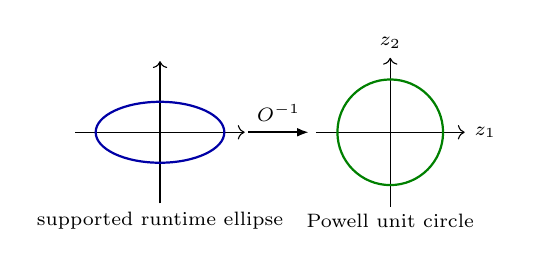
\begin{tikzpicture}[scale=0.86,
  every node/.style={font=\scriptsize},
  arr/.style={-{Latex[length=1.5mm]},thick}]
\begin{scope}[xshift=-1.65cm]
\draw[->] (-1.25,0)--(1.25,0);
\draw[->] (0,-1.05)--(0,1.05);
\draw[blue!65!black,thick] (0,0) ellipse (0.95 and 0.45);
\node at (0,-1.3) {supported runtime ellipse};
\end{scope}
\draw[arr] (-0.35,0)--(0.55,0) node[midway,above]{$O^{-1}$};
\begin{scope}[xshift=1.75cm]
\draw[->] (-1.1,0)--(1.1,0) node[right]{$z_1$};
\draw[->] (0,-1.1)--(0,1.1) node[above]{$z_2$};
\draw[green!50!black,thick] (0,0) circle (0.78);
\node at (0,-1.3) {Powell unit circle};
\end{scope}
\end{tikzpicture}
\end{center}

\conceptbreak

\section*{Part VI. The objective Powell actually evaluates}

\subsection*{The canonical fixed chart}

\micro Powell searches the complete accepted ansatz through one fixed linear
lift constructed at the zero-growth origin.

At this point the preceding maps become one callable objective. Powell itself
receives an \(r\)-component real vector \(z\) and returns proposals in that
coordinate space. A wrapper applies \(O\), \(P\), and \(R\), prepares the
corresponding quantum state, and evaluates the Hamiltonian energy. The
optimizer can therefore remain agnostic about binary padding, logical blocks,
metric support, and circuit indexing; those structures have already been
compiled into the fixed map from \(z\) to the executable runtime array.

\mathderiv Let \(\bm\phi^{(0)}\) be the complete accepted logical vector after
zero-angle admission. Construct \(P\), \(R\), \(G_\phi\), \(G_\vartheta\), and
\(O\) at the state
\begin{equation}
\ket{\psi^{(0)}}=U(R\bm\phi^{(0)})\ket{\psi_{\rm ref}}.
\label{eq:powell-origin}
\end{equation}
For every Powell trial \(z\in\R^r\), define
\begin{align}
\delta\bm\vartheta(z)&=Oz,\nonumber\\
\bm\phi(z)&=\bm\phi^{(0)}+POz,\nonumber\\
\widehat{\bm\vartheta}(z)&=R\bm\phi(z)
=R(\bm\phi^{(0)}+POz),\nonumber\\
\ket{\psi(z)}&=U(\widehat{\bm\vartheta}(z))
\ket{\psi_{\rm ref}},\nonumber\\
E(z)&=\bra{\psi(z)}H\ket{\psi(z)}.
\label{eq:powell-objective-chain}
\end{align}
The optimizer starts at
\begin{equation}
z^{(0)}=0,\qquad
\widehat{\bm\vartheta}(0)=R\bm\phi^{(0)},\qquad
E(0)=E^{(0)}.
\label{eq:powell-zero}
\end{equation}
At the origin,
\begin{equation}
\left\|\left.\frac{d}{d\epsilon}
\ket{\psi(\epsilon z)}\right|_{\epsilon=0,\perp}\right\|_{\R}^2
=z^{\mathsf T}z.
\label{eq:powell-origin-length}
\end{equation}

\begin{center}
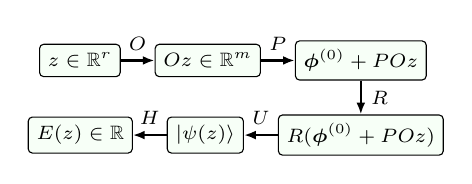
\begin{tikzpicture}[
  node distance=4.3mm,
  every node/.style={font=\scriptsize,align=center},
  box/.style={draw,rounded corners=1.5pt,inner sep=3pt,fill=green!3},
  arr/.style={-{Latex[length=1.5mm]},thick}
]
\node[box] (z) {$z\in\R^r$};
\node[box,right=of z] (rt) {$Oz\in\R^m$};
\node[box,right=of rt] (lg) {$\bm\phi^{(0)}+POz$};
\node[box,below=of lg] (ev) {$R(\bm\phi^{(0)}+POz)$};
\node[box,left=of ev] (psi) {$\ket{\psi(z)}$};
\node[box,left=of psi] (en) {$E(z)\in\R$};
\draw[arr] (z)--node[above]{$O$}(rt);
\draw[arr] (rt)--node[above]{$P$}(lg);
\draw[arr] (lg)--node[right]{$R$}(ev);
\draw[arr] (ev)--node[above]{$U$}(psi);
\draw[arr] (psi)--node[above]{$H$}(en);
\end{tikzpicture}
\end{center}

\commentaryblock Powell manipulates \(z\), and the chart wrapper carries out
all other maps for every objective call. The product \(PO\) converts the
supported physical coordinates into changes of all accepted logical angles.
Adding \(\bm\phi^{(0)}\) places those changes around the inherited accepted
state, and \(R\) expands the logical angles into the shared-entry runtime
array. The optimizer therefore explores the complete accepted logical ansatz
family through axes normalized by local physical state motion. Every admitted
generator participates because \(\bm\phi^{(0)}\) and the rows of \(PO\)
cover the complete logical registry.

\physical The Hamiltonian supplies the scalar landscape after each whitened
direction has been converted into an executable circuit. FS whitening
equalizes tangent length and leaves energetic stiffness for the objective to
reveal. A physically short, energetically steep direction and a physically
long, energetically flat direction receive comparable initial state-motion
scales in \(z\). Powell then samples finite displacements in these directions,
so the evaluated energy automatically includes nonlinear interference among
all accepted generators. The chart governs how the search moves through the
state manifold; the Hamiltonian governs which of those movements lower the
energy.

\conceptbreak

\subsection*{Why the chart is fixed for one Powell invocation}

\micro One anchor Gram matrix defines a coherent coordinate frame for the
entire finite Powell search.

\mathderiv Denote the origin metric by \(G_\vartheta^{(0)}\) and its
orthonormalizer by \(O^{(0)}\). The chart certificate is
\begin{equation}
(O^{(0)})^{\mathsf T}G_\vartheta^{(0)}O^{(0)}=I_r.
\label{eq:fixed-certificate}
\end{equation}
Every objective evaluation uses
\begin{equation}
z\longmapsto R\bigl(\bm\phi^{(0)}+PO^{(0)}z\bigr).
\label{eq:fixed-map}
\end{equation}
At a displaced point \(z\), the exact local metric in these coordinates is
\begin{equation}
G_z(z)=(O^{(0)})^{\mathsf T}P^{\mathsf T}
G_\phi(\bm\phi(z))P O^{(0)}.
\label{eq:evolving-local-metric}
\end{equation}
The origin identity is \(G_z(0)=I_r\). The next accepted admission creates a
new registry and a new origin, leading to
\begin{equation}
G_{\vartheta,k+1}^{(0)}
\longrightarrow (V_{k+1,+},\Lambda_{k+1,+})
\longrightarrow O_{k+1}^{(0)}.
\label{eq:next-chart}
\end{equation}

\commentaryblock The fixed map gives every Powell line search one common
coordinate meaning. Its orthonormality is exact at the accepted origin and
serves as a local preconditioner across the nonlinear trial set. The metric
\(G_\phi(\bm\phi(z))\) generally evolves as the circuit moves, as
Eq.~\eqref{eq:evolving-local-metric} records, yet each trial is expressed in
the same origin frame \(O^{(0)}\). This common frame makes line-search
coordinates comparable across objective calls. The next structural admission
changes the manifold registry by adding a logical block, so the next refit
receives a fresh tangent matrix, Gram matrix, support certificate, and
orthonormalizer.

\impl The Gram matrix is constructed once per accepted-refit Powell invocation.
All energy calls inside that invocation reuse \(O^{(0)}\), \(P\), and \(R\).
The word \emph{fixed} refers precisely to this lifetime: one zero-growth
origin, one FS Gram construction, one support decomposition, and one linear
chart serve the complete optimizer call. The metric-query charge therefore
belongs to chart construction, and the Powell objective calls contribute
Hamiltonian-energy evaluations. Telemetry records the raw logical metric, raw
expanded metric, retained rank, orthonormalizer, map hashes, origin state hash,
and identity residual. After the controller admits the next singleton, the
expanded registry and origin change, and the subsequent Powell invocation
constructs the next fixed chart.

\conceptbreak

\section*{Part VII. End-to-end canonical round}

\micro A single controller round joins legality, structural growth, projective
geometry, and derivative-free optimization in a fixed order.

Recall the three forms through which the admitted object has already passed.
It began as a raw Pauli proposal in the ambient qubit register, became a legal
grouped generator through exact projection, and acquired one zero-initialized
logical coordinate with an expanded runtime block. The accepted-refit chart
now supplies the fourth form: a mixture of supported orthonormal tangent
coordinates. Equation~\eqref{eq:complete-round} composes these forms into the
single controller-round map.

\mathderiv The end-to-end map can be written as
\begin{equation}
\begin{aligned}
\mathcal A_k
&\xrightarrow{\ \mathcal P(\cdot)\mathcal P\ }
\widetilde{\mathcal A}_k
\xrightarrow{\ \text{feasibility and selection}\ }
\widetilde A_{r_k},\\
(U_k,\bm\phi_k)
&\xrightarrow{\ \phi_{r_k}=0\ }
(U_{k,+},\bm\phi_{k,+}^{(0)}),\\
\bm\phi_{k,+}^{(0)}
&\xrightarrow{\ T_\phi\ }
G_{\phi,k}^{(0)}
\xrightarrow{\ P_k^{\mathsf T}(\cdot)P_k\ }
G_{\vartheta,k}^{(0)},\\
G_{\vartheta,k}^{(0)}
&\xrightarrow{\ \mathcal I_+\ }
(V_{k,+},\Lambda_{k,+})
\xrightarrow{\ V_{k,+}\Lambda_{k,+}^{-1/2}\ }
O_k,\\
z
&\xrightarrow{\ R_k(\bm\phi_{k,+}^{(0)}+P_kO_kz)\ }
\widehat{\bm\vartheta}_k(z)
\xrightarrow{\ U_{k,+},H\ }
E_k(z),\\
z_k^*&\in\operatorname*{arg\,min}_{z\in\R^{r_k}}E_k(z),\\
\bm\phi_{k+1}
&=\bm\phi_{k,+}^{(0)}+P_kO_kz_k^*.
\end{aligned}
\label{eq:complete-round}
\end{equation}

\subsection*{Invariant checklist}

Each arrow carries a distinct certificate. Together these certificates make
the construction replayable, because they verify the meaning of every
representation before the next map consumes it:
\begin{enumerate}[leftmargin=1.25em,itemsep=2pt,topsep=2pt]
\item \textbf{Legal action:}
\((I-\mathcal P)\widetilde A\mathcal P=0\).
\item \textbf{Zero growth:}
\(\ket{\psi_{k,+}^{(0)}}=\ket{\psi_k}\).
\item \textbf{Shared-angle registry:}
\(P_kR_k=I\) and
\(\widehat{\bm\vartheta}=R_kP_k\bm\vartheta\).
\item \textbf{Metric pullback:}
\(G_{\vartheta,k}=P_k^{\mathsf T}G_{\phi,k}P_k\).
\item \textbf{Support:}
\(\Lambda_{k,+}\succ0\) under the declared relative threshold.
\item \textbf{Whitening:}
\(O_k^{\mathsf T}G_{\vartheta,k}O_k=I\) within tolerance.
\item \textbf{Exact origin:}
\(z=0\) reproduces the inherited runtime array, state, and energy.
\item \textbf{Fixed invocation:}
one \(O_k\) serves every Powell objective call in the refit.
\item \textbf{Full scope:}
the logical registry contains every accepted generator.
\end{enumerate}

\physical These invariants divide the algorithm into auditable mechanisms
whose outputs feed one another. Legality controls the encoded Hilbert space and
thereby fixes the admissible generator. Shared-angle projection controls the
ansatz parameterization and thereby fixes how that generator appears in the
runtime array. FS support controls the physically resolved tangent quotient and
thereby fixes which mixtures can serve as optimization coordinates. Whitening
controls their numerical scale, and Powell supplies nonlinear energy descent
inside the complete accepted manifold. A replay that reproduces every
certificate has reconstructed the same route from operator admission through
objective evaluation.

\conceptbreak

\section*{Part VIII. What the chart changes and preserves}

\subsection*{Coordinate transformation of local models}

\micro Every differential and curvature tensor follows the same coordinate
map as the displacement it evaluates.

\mathderiv Let the supported logical displacement be
\begin{equation}
\delta\bm\phi=Wz,\qquad W=PO.
\label{eq:logical-whitened-map}
\end{equation}
For a local energy expansion
\begin{equation}
E(\bm\phi^{(0)}+\delta\bm\phi)
=E_0-g_\phi^{\mathsf T}\delta\bm\phi
+\frac12\delta\bm\phi^{\mathsf T}H_\phi\delta\bm\phi
+\mathcal O(\|\delta\bm\phi\|^3),
\label{eq:logical-energy-model}
\end{equation}
substitution gives
\begin{align}
E(z)
&=E_0-g_z^{\mathsf T}z
+\frac12z^{\mathsf T}H_zz
+\mathcal O(\|Wz\|^3),\nonumber\\
g_z&=W^{\mathsf T}g_\phi,\qquad
H_z=W^{\mathsf T}H_\phi W.
\label{eq:whitened-energy-model}
\end{align}
The scalar contractions are invariant:
\begin{align}
g_z^{\mathsf T}z
&=g_\phi^{\mathsf T}\delta\bm\phi,\nonumber\\
z^{\mathsf T}H_zz
&=\delta\bm\phi^{\mathsf T}H_\phi\delta\bm\phi.
\label{eq:model-invariance}
\end{align}

\commentaryblock Whitening changes the array used to describe a tangent. The
map \(W=PO\) carries each \(z\)-coordinate displacement into the corresponding
logical-angle displacement, and the gradient and Hessian transform by the
transpose and congruence relations in
Eq.~\eqref{eq:whitened-energy-model}. These transformations preserve the
linear and quadratic scalar contractions in
Eq.~\eqref{eq:model-invariance}; hence they preserve the represented tangent,
state family, energy function, and local scalar response. Powell's finite
evaluation budget can follow a distinct numerical path because its initial
direction set is now expressed in the orthonormal FS frame. The physical model
is held fixed, and the numerical search receives coordinates commensurate with
local state displacement.

\subsection*{A compact distinction map}

The following table gathers the construction by role. Reading downward
reproduces the same causal sequence as Eq.~\eqref{eq:architecture}: legal
operator construction, shared-coordinate representation, physical metric
measurement, supported whitening, and executable state preparation.

\begin{center}
\renewcommand{\arraystretch}{1.15}
\begin{tabular}{@{}p{0.28\columnwidth}p{0.64\columnwidth}@{}}
\toprule
Object & Role \\
\midrule
\(\mathcal P\) & selects legal encoded boson states and projects a raw child \\
\(P,R\) & connect expanded runtime entries and shared logical angles \\
\(G_\phi\) & measures FS tangent length in logical coordinates \\
\(G_\vartheta\) & represents the same metric after runtime pullback \\
\(V_+,\Lambda_+\) & certify the resolved positive tangent support \\
\(O\) & maps Powell coordinates to supported runtime displacements \\
\(PO\) & maps Powell coordinates to logical angle changes \\
\(R(\bm\phi^{(0)}+POz)\) & produces the executable shared-angle runtime array \\
\bottomrule
\end{tabular}
\end{center}

\conceptbreak

\section*{Post-Reading Mastery Quiz (Exit Quiz)}

For each question, record the strongest answer, the decisive reason, and a
confidence estimate. The questions test the construction developed in this
primer.

\subsection*{Conceptual judgment}

\textbf{1.} One projected singleton produces two runtime factors with one
shared logical angle. Which operation supplies the physical coordinate space
used by Powell?
\begin{enumerate}[label=\Alph*.,leftmargin=1.45em,itemsep=1pt,topsep=2pt]
\item Retain both runtime axes and normalize each diagonal Gram entry.
\item Average the block, pull back the complete FS metric, retain its positive
support, and orthonormalize that support.
\item Average the block once, then allow Powell to vary both factor angles
independently during line searches.
\item Retain the logical block mean and use the Euclidean logical coordinate
scale as the FS scale.
\end{enumerate}

\textbf{2.} Powell reaches a trial point far from the accepted origin. Which
statement matches the fixed-chart contract?
\begin{enumerate}[label=\Alph*.,leftmargin=1.45em,itemsep=1pt,topsep=2pt]
\item Rebuild the Gram matrix at every trial and express the next line search
in the newest frame.
\item Rebuild the Gram matrix after each successful Powell direction and retain
the accumulated coordinate vector.
\item Reuse the origin orthonormalizer for the complete invocation and build a
fresh chart after the next structural admission.
\item Reuse the origin eigenvalues and update the eigenvectors from every trial
state.
\end{enumerate}

\subsection*{Terminology and object roles}

\textbf{3.} In this construction, what is an expanded-runtime alias direction?
\begin{enumerate}[label=\Alph*.,leftmargin=1.45em,itemsep=1pt,topsep=2pt]
\item A runtime displacement in \(\ker P\) that preserves every logical block
mean and produces zero horizontal tangent motion.
\item A retained eigenmode whose FS eigenvalue is small relative to the energy
Hessian eigenvalue.
\item A projected Pauli component whose coefficient cancels a padding
transition at finite angle.
\item A logical displacement that changes the state and preserves its energy
to second order.
\end{enumerate}

\subsection*{Mathematical-form recognition}

\textbf{4.} Given \(\delta\bm\phi=P\delta\bm\vartheta\), which identity
represents the same FS quadratic form in expanded runtime coordinates?
\begin{equation*}
\begin{aligned}
\mathrm A\quad&G_\vartheta=P^{\mathsf T}G_\phi P,\\
\mathrm B\quad&G_\vartheta=PG_\phi P^{\mathsf T},\\
\mathrm C\quad&G_\vartheta=P^{-\mathsf T}G_\phi P^{-1},\\
\mathrm D\quad&G_\vartheta=R^{\mathsf T}G_\phi R.
\end{aligned}
\end{equation*}

\conceptbreak

\section*{Transfer-and-Repair Work}

Keep these problems unsolved and use the completed derivations as the source
for a later critique.
\begin{enumerate}[leftmargin=1.25em,itemsep=4pt,topsep=2pt]
\item For \(n_{\max}=2\), derive
\(\mathcal P_3(X_1I_0)\mathcal P_3\) in the two-qubit Pauli basis. Identify
the retained Fock-level transition and the runtime block size.
\item Consider one logical generator with three runtime factors. Construct its
row of \(P\), its column of \(R\), and an explicit two-dimensional basis for
the alias subspace inside that block.
\item Replace the diagonal \(G_\phi\) in Eq.~\eqref{eq:toy-logical-gram} by
\(\bigl[\begin{smallmatrix}4&1\\1&9\end{smallmatrix}\bigr]\). Predict which
parts of the derivation remain exact, then compute the new expanded Gram and
identify its alias eigenvector.
\item A proposed implementation rebuilds \(O\) after every Powell objective
call and leaves the optimizer coordinate vector unchanged. Diagnose the
coordinate inconsistency and specify the transformation required to preserve
the represented runtime displacement across a frame change.
\item Starting from Eq.~\eqref{eq:complete-round}, mark every operation that
requires quantum-measurement information and every operation that is a
classical linear-algebra transformation. Explain the resulting metric-query
accounting for one Powell invocation.
\end{enumerate}

\newpage
\section*{Detachable Solutions to the Mastery Quiz}

\textbf{1. B.} The block average defines the shared logical motion, the metric
pullback represents that motion in the expanded array, support selects the
resolved quotient, and \(O\) orthonormalizes its FS scale. Choice D omits the
state-dependent physical metric and therefore preserves a coordinate scale
whose relation to state-motion length remains uncertified.

\textbf{2. C.} The origin Gram matrix and \(O\) define one coordinate frame for
the complete Powell invocation. The next structural admission changes the
coordinate registry and supplies the next chart-construction event. Choice A
creates a sequence of frames and requires explicit coordinate transport after
every trial.

\textbf{3. A.} An alias is a runtime redistribution whose block averages vanish.
The chain \(a\in\ker P\Rightarrow T_\vartheta a=0\Rightarrow
G_\vartheta a=0\) gives its defining invariant. Choice C describes a Pauli
component participating in legal-subspace cancellation, which belongs to the
operator projection stage.

\textbf{4. A.} Substitution proves the pullback:
\begin{align*}
\delta\bm\phi^{\mathsf T}G_\phi\delta\bm\phi
&=(P\delta\bm\vartheta)^{\mathsf T}G_\phi
(P\delta\bm\vartheta)\\
&=\delta\bm\vartheta^{\mathsf T}
(P^{\mathsf T}G_\phi P)\delta\bm\vartheta.
\end{align*}
Choice B has logical-space shape because its outer dimensions equal the row
dimension of \(P\).

\section*{Canonical implementation anchors}

The mathematical construction corresponds to these stable executable
identities:
\begin{itemize}[leftmargin=1.25em,itemsep=2pt,topsep=2pt]
\item route family: \path{singleton_response_snake};
\item Powell base chart:
\path{expanded_runtime_projected_logical_v1};
\item accepted-refit scope: \path{full_ansatz_v1};
\item accepted-refit chart:
\path{supported_fs_whitened_fixed_v1};
\item binary-padding child policy:
\path{exact_projected_grouped_v1};
\item parameterization mode: \path{logical_shared};
\item chart lifetime: one accepted-refit Powell invocation.
\end{itemize}

The primary implementation surfaces are
\begin{itemize}[leftmargin=1.25em,itemsep=2pt,topsep=2pt]
\item \path{pipelines/static_adapt/route_a_child_padding.py},
\item \path{pipelines/static_adapt/accepted_refit.py},
\item \path{src/quantum/ansatz_parameterization.py},
\item \path{pipelines/static_adapt/joint_linear_solve.py}.
\end{itemize}

\section*{Dimensional audit and reconstruction recipe}

Let \(d\) be the number of accepted logical generators, \(m\) the number of
expanded runtime entries, and \(r\) the retained FS support rank. The canonical
objects have the following typed dimensions:
\begin{center}
\renewcommand{\arraystretch}{1.13}
\begin{tabular}{@{}ll@{}}
\toprule
Object & Shape or map \\
\midrule
\(\bm\phi\) & \(\R^d\) \\
\(\bm\vartheta\) & \(\R^m\) \\
\(P\) & \(\R^m\to\R^d\) \\
\(R\) & \(\R^d\to\R^m\) \\
\(T_\phi\) & \(\R^d\to T_{[\psi]}\mathcal M\) \\
\(G_\phi\) & \(d\times d\) \\
\(G_\vartheta=P^{\mathsf T}G_\phi P\) & \(m\times m\) \\
\(V_+\) & \(m\times r\) \\
\(\Lambda_+\) & \(r\times r\) \\
\(O=V_+\Lambda_+^{-1/2}\) & \(\R^r\to\R^m\) \\
\(PO\) & \(\R^r\to\R^d\) \\
\bottomrule
\end{tabular}
\end{center}
The rank inequalities
\begin{equation}
r\leq\rank G_\vartheta\leq\rank P=d\leq m
\label{eq:dimension-ranks}
\end{equation}
encode two possible reductions. Shared-angle aliases enter through
\(\ker P\). Additional physical tangent dependencies enter through
\(\ker T_\phi\). Spectral support resolves their combined metric-null space.

\paragraph{Reconstruction from one preserved checkpoint.}
A complete replay reads the accepted logical registry and runtime slices,
forms \(P\) and \(R\) from those slices, prepares the zero-growth state,
constructs every horizontal accepted tangent, and builds \(G_\phi\). It then
computes \(G_\vartheta=P^{\mathsf T}G_\phi P\), applies the recorded relative
support threshold, and forms \(O=V_+\Lambda_+^{-1/2}\). The numerical
certificates are
\begin{align}
\|PR-I_d\|&\leq\epsilon_{\rm map},\nonumber\\
\|O^{\mathsf T}G_\vartheta O-I_r\|
&\leq\epsilon_{\rm white},\nonumber\\
\|R(\bm\phi^{(0)}+PO0)-R\bm\phi^{(0)}\|&=0.
\label{eq:reconstruction-certificates}
\end{align}
These checks connect serialized operator blocks to the fixed objective
\(E(z)\) that Powell receives.

\end{document}
